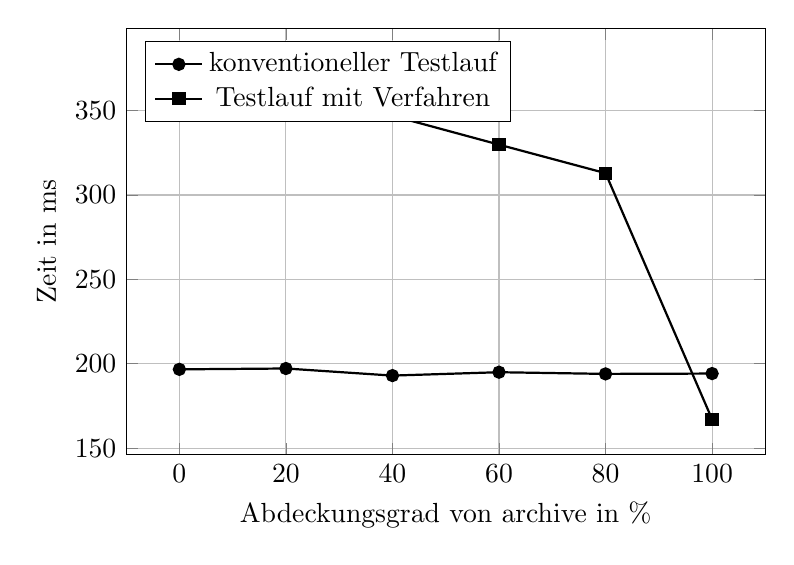
\begin{tikzpicture}
    \begin{axis}[
        width=0.8\textwidth,
        height=7cm,
        xlabel={Abdeckungsgrad von archive in \%},
        ylabel={Zeit in ms},
        grid=major,
        legend pos=north west
    ]
    \addplot[
        thick,
        mark=*,
    ] coordinates {
        (0, 196.7)
        (20, 197.2)
        (40, 193.0)
        (60, 195.0)
        (80, 194.0)
        (100, 194.2)
    };
    \addlegendentry{konventioneller Testlauf}
    \addplot[
        thick,
        mark=square*,
    ] coordinates {
        (0, 377.7)
        (20, 363.9)
        (40, 346.9)
        (60, 329.8)
        (80, 312.9)
        (100, 167.1)
    };
    \addlegendentry{Testlauf mit Verfahren}
    \end{axis}
\end{tikzpicture}
